\chapter{神经回路介导行为的神经解剖学基础} \label{chap:chap4}

人脑执行任务的方式是当前任何计算机都无法企及的。
仅仅是看世界并识别一张脸或面部表情就需要惊人的计算成就。
事实上,我们所有的感知能力,包括视、听、嗅、味和触摸,都是分析的胜利。
同样,我们所有的自发行动都是工程学的胜利。
感知和运动本身虽然奇妙,但与形成记忆或理解社会规范等复杂认知行为相比,就显得相形见绌了。


大脑之所以能完成这些计算壮举,是因为其神经细胞以非常精确的功能回路相互连接。
大脑呈层级组织结构,使得在一个层级处理的信息能传递给更高级别的回路进行更复杂精细的处理。 
从本质上讲,大脑是一个网络的网络。 
不同大脑区域以集成的方式协同工作,以实现有目的的行为。


在本章中,我们将概述一些使大脑能够处理感觉输入并产生运动输出的神经解剖组织回路。
我们特别关注触觉作为一种感觉模式,因为躯体感觉系统被特别透彻地研究过,并且触觉清晰地展示了从脊髓到大脑皮层等多个层次上感觉处理回路的交互作用。
我们在这里的目的是说明回路如何控制行为的基本原理。 
在下一章中,我们将考虑这些回路的功能特性,包括它们处理信息的计算。 
在随后的章节中,我们将更详细地讨论各种感觉方式的解剖结构和功能,以及感觉输入如何调节运动。


最后,我们提供了大脑回路的预览,这些回路有助于产生我们日常生活的记忆,称为外显记忆(见第~\ref{chap:chap52}~章和第~\ref{chap:chap54}~章)。
我们这样做是为了说明:
虽然记忆回路中的许多神经元与感觉和运动回路中的神经元相似,但并非所有神经元都相似。
此外,记忆系统中回路之间的路径组织与运动和感觉系统中的组织不同。
这突显了一个基本的神经生物学原则,即大脑的不同回路已经进化出了最有效执行特定功能的组织结构。


理解大脑的功能组织乍一看似乎令人生畏。 
但正如我们在前一章中看到的那样,大脑的组织通过三个解剖学考虑得到了简化。
首先,神经元的\textit{种类}相对较少。
成千上万的脊髓运动神经元或数百万个新皮层锥体细胞中的每一个都具有相似的解剖结构并具有相似的功能。 
其次,大脑和脊髓中的神经元\textit{聚集}在称为核或大脑皮层离散区域的功能组中,形成网络或功能系统。 
第三,大脑皮层的离散\textit{区域}专门负责感觉、运动或记忆等联想功能。


\section{局部回路执行特定的神经计算,协调这些计算以调制复杂的行为}

神经元相互连接形成功能回路。 
例如,在脊髓内,简单的反射回路接收来自牵张受体的感觉信息,并向不同的肌肉群发送输出。
对于更复杂的功能性行为,信息处理的不同阶段在神经系统不同区域的网络中进行。
神经系统内神经元之间的连接可以有不同的长度。


在大脑某个区域内,局部连接(可能是兴奋性的或抑制性的)将许多神经元整合成功能网络。
这些局部网络随后可能通过更长的投射为一个或多个其他大脑区域提供输出。
这些较长的路径中有许多都有特定名称。
例如,从丘脑的外侧膝状体核到视觉皮层的投射称为\textit{视辐射}。
从大脑一侧的皮层到大脑另一侧皮层(大脑皮层中最靠近大脑表面的区域)的连接形成了胼胝体。
如图~\ref{fig:4_1}~所示,这些长通路携带的信息整合了许多局部回路的输出。


\begin{figure}[htbp]
	\centering
	\includegraphics[width=1.0\linewidth]{chap04/fig_4_1}
	\caption{背柱-内侧丘系通路是体感信息的主要传入通路。 
		体感信息通过背根神经节细胞进入中枢神经系统。 
		信息流最终通向体感皮层。 
		来自身体不同部位的传递信息的纤维之间保持着有序的关系,并在其每个突触中止的模式中形成了身体表面的神经映射图。}
	\label{fig:4_1}
\end{figure}


如图~\ref{fig:4_2}~所示,考虑一下击打网球的简单动作。
关于来球运动的视觉信息在视觉系统中被分析,这是一个从视网膜延伸到丘脑的外侧膝状体,再到枕叶和颞叶数十个皮层区域的分级组织系统(第~\ref{chap:chap21}~章)。
这些信息在运动皮层与关于手臂、腿部和躯干位置的本体感觉信息相结合,计算出拦截球所需的运动。 
一旦挥拍开始,基于关于来球轨迹和手臂位置的持续感官信息流,大脑中其他专门负责运动的区域,如小脑,会对运动程序做出许多微调。


\begin{figure}[htbp]
	\centering
	\includegraphics[width=1.0\linewidth]{chap04/fig_4_2}
	\caption{一个简单的行为是由大脑的许多部分调节的。 
		A. 一名网球运动员在观看接近的球时使用视觉皮层来判断球的大小、方向和速度。 
		而前运动皮层则会制定出一个动作程序以回应击球。
		与此同时,杏仁核与其他大脑区域协作,调节心率、呼吸和其他\textit{内稳态}机制,并激活下丘脑,激发选手击球的良好动机。 
		B. 要完成这一击球动作,选手必须动用A部分中提到的所有结构,以及其他一些结构。
		运动皮层向脊髓发出信号,激活和抑制手臂和腿部的许多肌肉。
		基底神经节开始参与启动运动模式,并可能回忆起学习的动作以正确击球。
		小脑根据来自外周感觉受体的本体感受信息调整运动。
		后顶叶皮层给予选手空间定位感,让他知道自己身体在空间中的位置以及球拍相对于身体的位置。
		脑干神经元在整个动作过程中调节心率、呼吸和唤醒水平。
		海马体并不直接参与击球过程,但它参与存储这次击球的记忆,以便选手稍后可以夸耀此事。}
	\label{fig:4_2}
\end{figure}


像大多数运动行为一样,击打网球并不是硬编码在大脑回路中,而是需要学习和记忆。
对运动任务的记忆,被称为程序性或内隐记忆,需要对运动皮层、基底核和小脑中的回路进行修改。
最后,整个行为是可以被意识所触及的,并可能引发对过去相似经历的有意识回忆,这被称为外显记忆,以及情绪反应。 
外显记忆取决于海马体中的回路(第~\ref{chap:chap52}~和~\ref{chap:chap54}~章),而情绪则由杏仁核(第~\ref{chap:chap42}~和~\ref{chap:chap53}~章)和部分眶额皮层、扣带回和岛叶皮层调节。
当然,在挥拍执行的过程中,大脑也在通过同样复杂的网络协调球员的心率、呼吸和其他内稳态功能。



\section{体感系统中的感官信息回路}

复杂的行为,例如区分抓球和抓书所需的运动行为,需要多个核和皮层区域的综合行动。
信息在大脑中以分层方式处理。
因此,有关刺激的信息通过一系列皮层下区域,然后是皮层区域传递; 
在每个处理级别,信息变得越来越复杂。


此外,即使是单一感官模式内的不同类型信息,也会在几个解剖学上分离的通路中被处理。
在体感系统中,对同一皮肤区域的轻触和针刺疼痛是由皮肤中连接到大脑中不同通路的不同感觉受体介导的。 
用于精细触觉、压力和本体感觉的系统称为\textit{精细觉系统},而用于疼痛和温度的系统称为\textit{粗感觉系统}。



\subsection{来自躯干和四肢的体感信息被传送到脊髓}

如图~\ref{fig:4_3}~所示,来自躯干和四肢的各种形式的体感信息进入脊髓,脊髓有一个核心的 H 形灰质区域,神经元细胞体位于该区域。 
灰质周围由髓鞘化的轴突构成的白质组成,这些轴突形成短连接和长连接。
脊髓两侧的灰质分为背角(或后角)和腹角(或前角)。


\begin{figure}[htbp]
	\centering
	\includegraphics[width=0.7\linewidth]{chap04/fig_4_3}
	\caption{脊髓的主要解剖学特征。 
		\textit{腹角}(绿色)包含较大的\textit{运动神经元},而\textit{背角}(橙色)包含较小的神经元。
		\textit{薄束}的纤维携带来自下肢的体感信息,而\textit{楔形束}的纤维携带来自上身的体感信息。
		\textit{侧柱}和\textit{腹柱}的纤维束包括上行和下行纤维束。}
	\label{fig:4_3}
\end{figure}


背角包含次级感觉神经元(感觉核),其树突从支配身体皮肤、肌肉和关节的初级感觉神经元接收刺激信息。
腹角包含运动神经元组(运动核),其轴突离开脊髓并支配骨骼肌。
脊髓具有介导从牵张反射到肢体运动协调等行为的回路。


如图~\ref{fig:3_5}~所示,正如我们在第~\ref{chap:chap3}~章中讨论的那样,在考虑膝跳反射时,灰质中各种类型的中间神经元调节脊髓运动神经元的输出。 
这些中间神经元中的一些是兴奋性的,而另一些是抑制性的。
这些中间神经元既调节流向大脑的感觉信息,也调节从大脑向下传至脊髓运动神经元的运动指令。
运动神经元也能通过中间神经元调整其它运动神经元的输出。
当我们在第~\ref{chap:chap32}~章讨论脊髓时,将更详细地考虑这些回路。


灰质周围的白质包含成束的上行轴突和下行轴突,它们分为背侧柱、侧柱和腹侧柱。
如图~\ref{fig:4_1}~所示,位于灰质两个背角之间的背柱仅包含将体感信息传递到脑干的上行轴突。
如图~\ref{fig:4_3}~所示,侧柱包括来自脑干和新皮层的上行和下行轴突,它们支配脊髓中间神经元和运动神经元。 
这证明了关于中枢神经系统连接的一般原则。
处理往往是分层的:
从低级到高级处理区域的投射称为前馈,而下行投射可以调节脊髓反射,被认为是反馈。 
区域A投射到区域B,同时B又向A返回投射的模式,在神经系统中反复出现。
腹侧柱还包括上行和下行轴突。 
侧柱和腹侧柱中的上行体感轴突构成并行通路,将有关疼痛和热感觉的信息传递到中枢神经系统的更高水平。 
下行轴突控制轴向肌肉和姿势。


如图~\ref{fig:4_4}~所示,脊髓沿其长度分为四个主要区域:颈椎、胸椎、腰椎和骶椎。
源自这些区域的连接根据胚胎期的体节而隔离,体节是肌肉、骨骼和身体其他组成部分发育的基础(第~\ref{chap:chap45}~章)。 
脊髓投射到在相同节段水平发育的身体结构的轴突,与穿过椎间孔进入脊髓的轴突结合形成脊神经。
颈椎水平的脊神经参与头部后部、颈部和手臂的感官知觉及运动功能;
胸椎水平的神经支配上躯干部;腰椎和骶骨脊神经则支配下躯干、背部和腿部。


\begin{figure}[htbp]
	\centering
	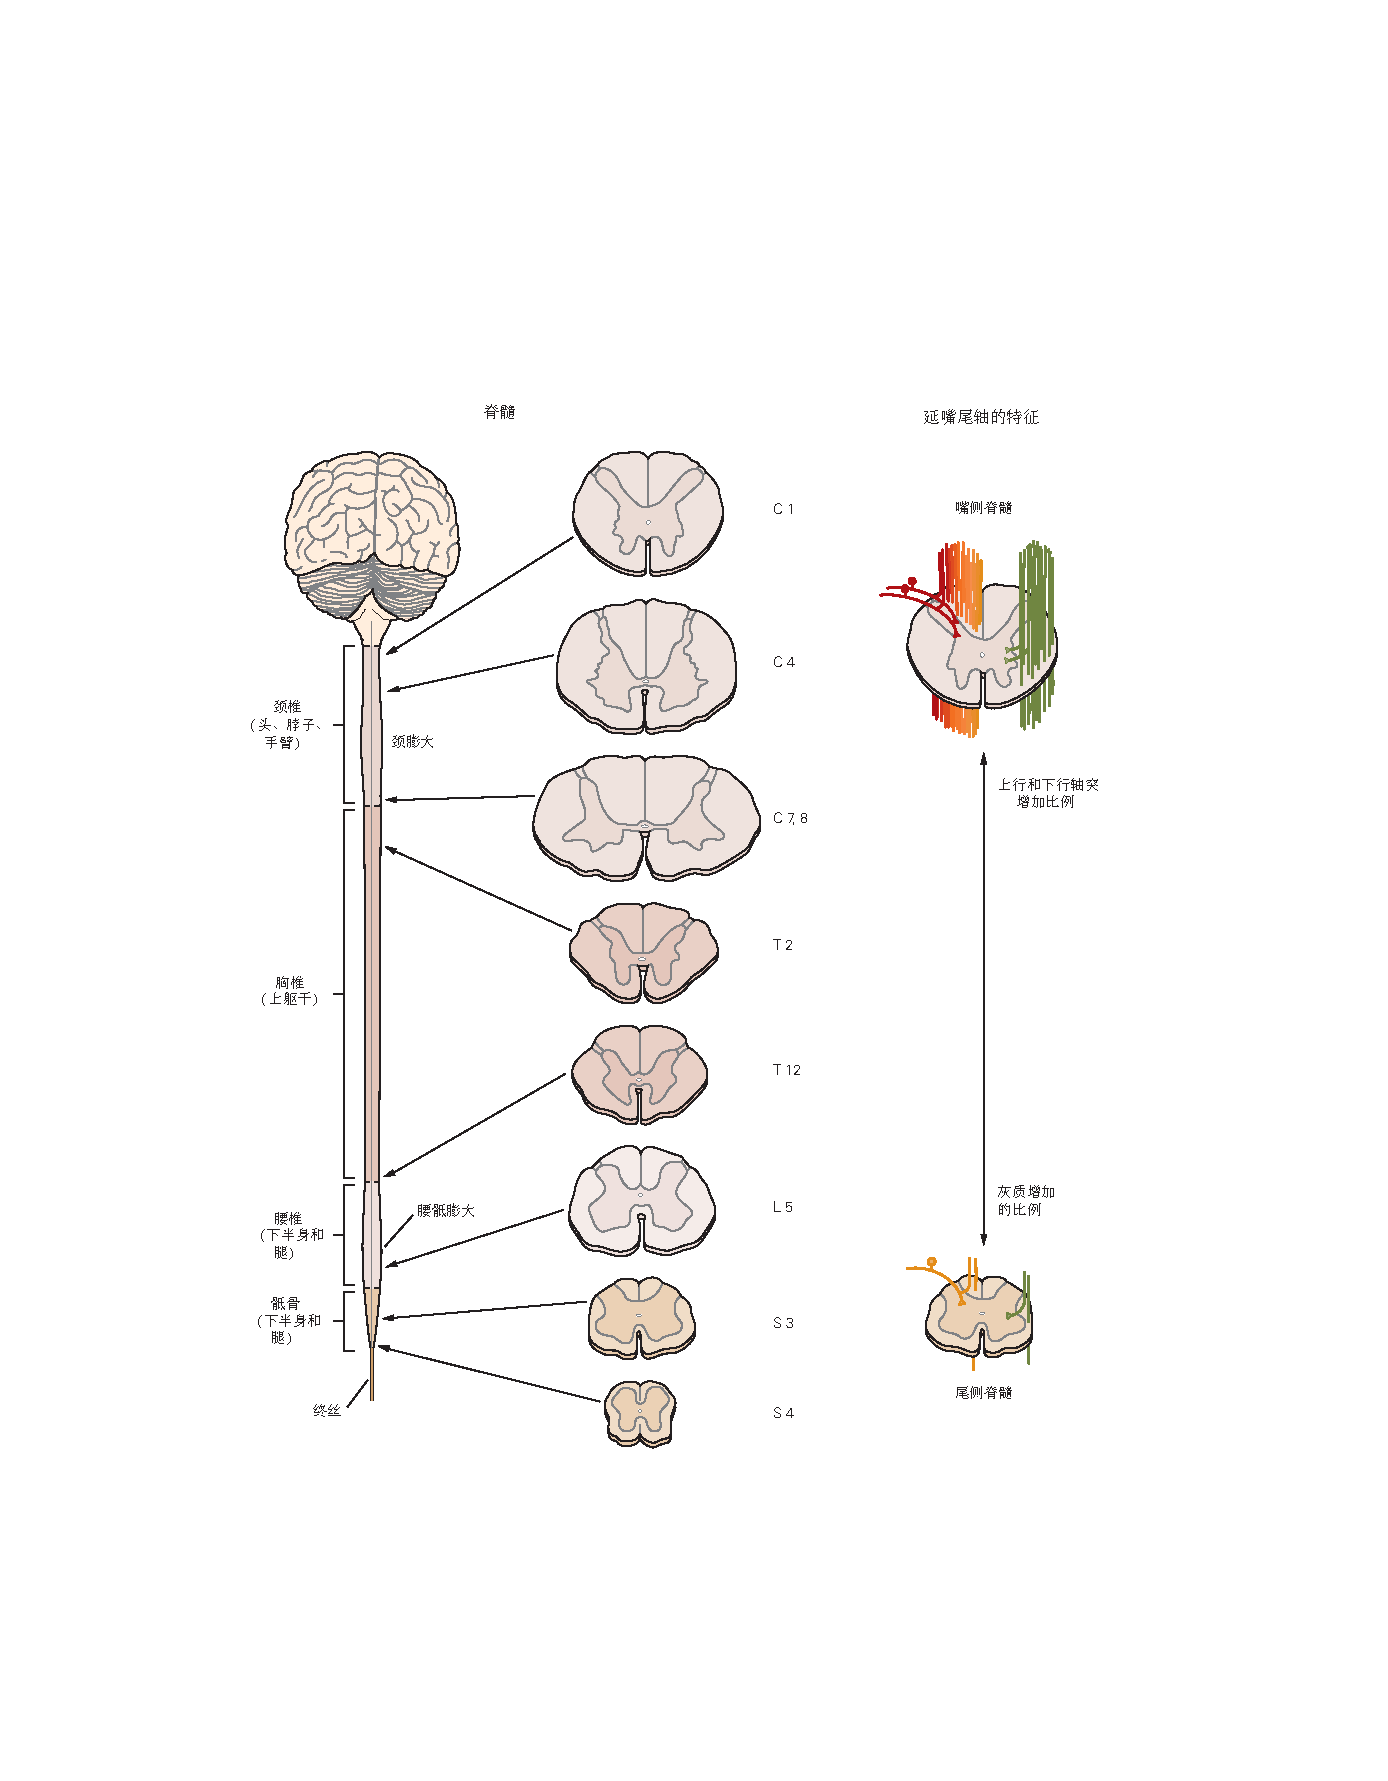
\includegraphics[width=1.0\linewidth]{chap04/fig_4_4}
	\caption{脊髓的内部和外部外观在不同的水平上有所不同。
		\textit{骶骨}水平的灰质(脊髓内的 H 形区域)与白质的比例大于\textit{颈椎}水平。
		在\textit{骶骨}水平,很少有传入的感觉轴突与脊髓相连,而大多数运动轴突已经终止于脊髓的更高水平。
		\textit{腰椎}和\textit{颈椎}水平的横截面增大是支配四肢的大量纤维进入或离开脊髓的区域。}
	\label{fig:4_4}
\end{figure}


脊髓的四个区域中,每一个都包含多个节段,大致对应于各自区域中不同椎骨的数量;
有8个颈段,12个胸段,5个腰段,5个骶段。
成熟的脊髓实质本身看起来并不分节,但四个脊髓区域的节段由进入或离开脊髓的背根和腹根的数量及位置来定义。
脊髓沿其头尾轴的大小和形状变化,是由于两种组织特征造成的。


% First, relatively few sensory axons enter
如图~\ref{fig:4_4}~所示,首先,在骶骨进入脊髓的感觉轴突相对较少。
随着脊髓节段逐渐升高(腰椎、胸椎、颈椎),进入脊髓的感觉轴突数量逐渐增加。
相反,多数来自大脑的下行轴突在颈椎终止,而向下至脊髓较低节段的下行轴突越来越少。
因此,白质中的纤维数量在颈椎水平最高(上行和下行纤维数量最多),而在骶骨水平最低。
因此,脊髓骶骨层的白质比灰质少得多,而颈髓的白质多于灰质。


如图~\ref{fig:4_4}~所示,第二个组织特征是腹角和背角大小的差异。
在支配手臂和腿部的运动神经所在的节段,腹角较大。
专用于身体区域的腹侧运动神经元的数量大致与该区域运动的灵巧性相当。
因此,与躯干相比,需要更多的运动神经元来支配更多肌肉以及调节肢体中更为复杂的运动。
同样,从肢体进入脊髓的感觉神经较多的部位,背角也较大。
肢体具有更高密度的感觉受体以介导更精细的触觉辨别,因此向脊髓发送更多的感觉纤维。
这些脊髓区域被称为腰骶扩大部和颈扩大部。



\subsection{躯干和四肢的初级感觉神经元聚集在背根神经节}

如图~\ref{fig:4_5}~所示,将信息从四肢和躯干的皮肤、肌肉和关节传递到脊髓的感觉神经元聚集在脊柱内的背根神经节中,紧邻脊髓。
这些神经元的形状是伪单极的;
它们有一个带有中央和外围分支的分叉轴突。
周围分支作为游离神经末梢支配皮肤、肌肉或其他组织,或与用于感知触觉、本体感觉(拉伸受体)、疼痛和温度的专门受体相关联。


\begin{figure}[htbp]
	\centering
	\includegraphics[width=0.65\linewidth]{chap04/fig_4_5}
	\caption{\textit{背根神经节}和脊神经根。
		从\textit{皮肤、肌肉和关节}获取感觉信息的神经元细胞体位于\textit{背根神经节},即与脊髓相邻的细胞簇。
		这些神经元的轴突分为外围和中央分支。 
		中央分支进入脊髓的背侧部分。}
	\label{fig:4_5}
\end{figure}


体感系统及其从受体到知觉的通路在第~\ref{chap:chap17}~章到第~\ref{chap:chap20}~章中有更全面的描述。
在这一点上,基本上有两条来自外围的体感通路,它们要么携带触摸和拉伸(精细觉系统),要么携带疼痛和温度(粗感觉系统)。
如图~\ref{fig:4_6}~所示,精细觉纤维在后柱-内侧丘系系统中移动。
来自背根神经节神经元的中央定向轴突在背(或后)柱白质中上行并终止于髓质的薄束核或楔束核。
疼痛和温度通路的中枢轴突形成脊髓丘脑通路。
它们终止于脊髓背角的灰质内。
如图~\ref{fig:4_6}~所示,二级神经元穿过脊髓的另一侧并在脊髓丘脑前束和侧束中上行。 
两条通路最终都终止于丘脑,丘脑将投射发送到大脑皮层的初级体感区域。
在下一节中,我们将重点关注\textit{精细觉系统}。


\begin{figure}[htbp]
	\centering
	\includegraphics[width=0.98\linewidth]{chap04/fig_4_6}
	\caption{来自四肢和躯干的体感信息通过两条上行通路传递到丘脑和大脑皮层。
		沿着从脊髓到大脑的神经轴的脑切片说明了将体感信息传递到大脑皮层的两条主要通路的解剖结构。
		这两条通路在到达脑桥之前是分开的,它们在那里并列。 背柱-内侧丘系系统(橙色)。
		触摸和肢体本体感觉信号通过大直径有髓神经纤维传递到脊髓和脑干,并在该系统中传递到丘脑。
		在脊髓中,用于触觉和本体感觉的纤维分开,一个分支进入同侧脊髓灰质,另一个在同侧背柱中上行到髓质。 
		来自背柱核神经元的二级纤维在髓质中穿过中线并在对侧内侧丘系中上行至丘脑,在那里它们终止于外侧和内侧腹侧后核。
		这些核中的丘脑神经元将触觉和本体感受信息传递给初级体感皮层。
		前外侧系统(棕色)。
		疼痛、瘙痒、温度和内脏信息通过终止于同侧背角的小直径有髓和无髓纤维传递到脊髓。
		该信息由脊髓内的神经元通过中线传递,并传递到对侧前外侧系统中的脑干和丘脑。
		终止于脑干的前外侧纤维组成脊髓网状束和脊髓中脑束; 剩余的前外侧纤维形成脊髓丘脑束。}
	\label{fig:4_6}
\end{figure}


来自触觉和本体感觉神经元的局部和上行分支为体感信息从背根神经节细胞进入脊髓提供了两条功能通路。 
局部分支可以激活调节运动输出的局部反射回路,而上行分支将信息传送到大脑,这些信息在丘脑和大脑皮层中进一步处理。



\subsection{脊髓中背根神经节神经元的中央轴突末端产生体表图}

背根神经节细胞的中央轴突终止于脊髓的方式形成了体表的神经图谱。
来自身体表面不同部分的输入的这种有序的躯体分布在整个上行的体感通路中保持不变。
这种排列说明了神经组织的另一个重要原则。
在任何特定水平上构成神经回路的神经元通常以系统的方式连接并且在个体之间看起来相似。 
同样,连接神经系统不同层次不同处理区域的纤维束也以高度组织化和模式化的方式排列。


进入骶骨区脊髓的轴突在靠近中线的背柱中上行,而那些依次进入更高水平的轴突在背柱内逐渐向外侧位置上行。 
因此,在颈髓中,来自身体所有部分的轴突已经进入,来自下半身的感觉纤维位于背柱的内侧,而来自躯干、手臂和肩部,最后是颈部的纤维逐渐占据更多 横向区域。 
如图~\ref{fig:4_1}~所示,在颈脊髓中,形成背柱的轴突分为两束:位于内侧的纤细束和位于更外侧的楔形束。



\subsection{每个躯体亚模态都在从外围到大脑的不同子系统中处理}

躯体感觉的\textit{亚模态}(触觉、痛觉、温度觉和位置觉)在大脑中通过终止于不同大脑区域的不同通路进行处理。
我们通过接触亚模态的信息路径来说明这些并行通路的特殊性。


携带触觉信息的初级传入纤维进入同侧背柱并上行到髓质。
来自下半身的纤维在细束中运行并终止于细核,而来自上半身的纤维在楔形束中运行并终止于楔形核。 
如图~\ref{fig:4_1}~所示,纤细核和楔形核中的神经元产生轴突,轴突穿过大脑的另一侧并在称为内侧丘系的长纤维束中上行到丘脑。


与脊髓的背柱一样,内侧丘系的纤维按体表排列。
因为携带感觉信息的纤维穿过中线到达大脑的另一侧,大脑的右侧接收来自身体左侧的感觉信息,反之亦然。 
如图~\ref{fig:4_1}~所示,内侧丘系的纤维终止于丘脑的特定部分,称为腹侧后外侧核。 
在那里,纤维保持它们的躯体组织,使得那些从下半身传递信息的纤维在横向结束,而那些从上半身传递信息的纤维在中间终止。



\section{丘脑是感觉受体和大脑皮层之间的重要纽带}

丘脑是一个蛋形结构,构成间脑的背侧部分。 
它包含一类称为丘脑中继细胞的兴奋性神经元,可将感觉输入传递到大脑皮层的初级感觉区域。 
然而,丘脑不仅仅是一个中继站。 
它充当信息到大脑皮层的守门人,根据生物体的行为状态阻止或增强特定信息的传递。


大脑皮层的反馈投射部分终止于丘脑的一个特殊部分,称为丘脑网状核。 
这个细胞核在丘脑周围形成一层薄片,几乎完全由突触到中继细胞上的抑制性神经元组成。 
它根本不投射到新皮层。 
除了接受来自新皮层的反馈投射外,网状核还接收来自离开丘脑前往新皮层的轴突的输入,使丘脑能够调节其中继细胞对传入感觉信息的反应。


丘脑是一个很好的例子,大脑区域由几个明确定义的核组成。
如图~\ref{fig:4_7}~所示,已识别出多达 50 个丘脑核团。
一些细胞核接收特定于感觉方式的信息并投射到新皮层的特定区域。
例如,如图~\ref{fig:4_1}~和图~\ref{fig:4_7}~所示,腹侧后外侧核(内侧丘系终止处)中的细胞处理体感信息,它们的轴突投射到初级体感皮层。 
如图~\ref{fig:4_7}~所示,从视网膜神经节细胞的投射终止于丘脑的另一部分,称为外侧膝状体核。 
该核中的神经元依次投射到视觉皮层。 
丘脑的其他部分参与运动功能,将信息从小脑和基底神经节传递到额叶的运动区域。 
自丘脑细胞并投射到新皮层的轴突在辐射冠中行进,这是一个大的纤维束,承载了大部分往返于大脑半球的轴突。。 
通过与额叶和海马体的联系,丘脑可能在记忆等认知功能中发挥作用。 
一些可能在注意力中起作用的核团广泛地投射到大而明显不同的皮层区域。


\begin{figure}[htbp]
	\centering
	\includegraphics[width=1.0\linewidth]{chap04/fig_4_7}
	\caption{丘脑的主要部分。
		丘脑是感觉信息从外周受体流向新皮层的关键中继站。
		体感信息从\textit{背根神经节}传递到丘脑\textit{腹后外侧核},然后从那里传递到\textit{初级体感皮层}。
		同样,来自\textit{视网膜}的视觉信息到达外侧膝状体核,从那里传递到枕叶的初级\textit{视觉皮层}。
		除嗅觉外,每个感觉系统在丘脑的不同区域内都有类似的处理步骤。}
	\label{fig:4_7}
\end{figure}


% The nuclei of the thalamus are most
如图~\ref{fig:4_7}~所示,丘脑的细胞核最常见的分为四组:相对于\textit{内髓板}的\textit{前侧}、\textit{内侧}、\textit{腹外侧}和\textit{后侧},一种片状纤维束,贯穿丘脑的尾部长度。
因此,内侧核团位于髓内板的内侧,而腹外侧核和后核核位于其外侧。
在丘脑的喙极,\textit{内髓板}分裂并包围前部。
丘脑的尾极被后组占据,以枕核为主。
纤维内部髓板中也分布着神经元群,它们统称为内髓板内核。


前组的主要输入来自下丘脑的乳头体核和海马体结构的前下托。 
前组的功能尚不明确,但由于其连接,认为它与记忆和情感有关。
前组主要与扣带回和额叶皮层区域相互连接。


内侧组主要由内侧核组成。 
这个大的丘脑核分为三个部分,每个部分都与额叶皮层的特定部分相连。 
细胞核接收来自基底神经节、杏仁核和中脑部分的输入,并与记忆和情绪处理有关。


腹外侧核的命名是根据它们在丘脑内的位置命名的。 
腹侧前核和腹侧核对运动控制很重要,并将信息从基底神经节和小脑传递到运动皮层。
腹侧后核将体感信息传递给新皮层。
如前所述,腹后外侧核传递来自脊髓束的信息。
腹后内侧核传递来自面部的信息,主要通过三叉神经(第 5 对颅神经)进入脑干。


后组包括内侧和外侧膝状体核、外侧后核和枕核。 
内侧膝状体是听觉系统的一个组成部分,根据其输入携带的声音频率信息按音调组织; 它将听觉信息传递到颞叶颞上回的初级听觉皮层。 
外侧膝状体接收来自视网膜的信息并将其传送到枕叶的初级视觉皮层。 
与啮齿类动物相比,灵长类大脑中的枕骨不成比例地扩大,尤其是在人类大脑中,其发育似乎与顶叶、枕叶和颞叶皮层联合区域的扩大并行。
它至少被分为三个亚区,并与顶叶、颞叶和枕叶的广泛区域以及与视觉相关的脑干的上丘和其他核团广泛互连。


如前所述,丘脑不仅投射到新皮层(前馈连接),而且还接收来自新皮层的广泛反馈输入(反馈连接)。 
例如,在外侧膝状核中,由视觉皮层反馈投射的轴突形成的突触数量实际上超过了外侧膝状体核从视网膜接收到的突触数量! 
这种反馈被认为在感觉信息处理中发挥重要的调节作用,尽管其确切功能尚未完全明了。
尽管这种反馈主要来自受两只眼睛激活的皮层神经元,但外侧膝状体核中的神经元仅响应一只眼睛或另一只眼睛。 
这意味着它们主要是由来自视网膜(来自不同层的不同眼睛)的输入驱动的,而不是来自皮层的反馈,尽管它在数量上有优势。 
丘脑的大多数核团从大脑皮层接收到类似显著的返回投射,这些投射的意义是神经科学未解之谜之一。


到目前为止描述的丘脑核团被称为中继(或特定)核团,因为它们与大脑皮层的特定部分有着特定且选择性的关系。其他称为非特异性核团的丘脑核团,则向多个皮层和皮层下区域投射。
这些核位于丘脑的中线(中线核)或内髓层内(板内核)。 
最大的中线核是室旁核、脑旁核和\textit{连结核};
最大的层内细胞群是中央核。 
椎板内核投射到内侧颞叶结构,如杏仁核和海马体,但也投射到部分基底神经节。
这些核从脊髓、脑干和小脑中的各种来源接收输入,并被认为可以调节皮层觉醒。


丘脑是感觉处理层次结构中的重要一步,它不是一个信息简单传递给大脑皮层的被动中继站。 
如图~\ref{fig:4_1}~所示,它是一个复杂的大脑区域,在这里进行大量信息处理。 
仅举一个例子,来自腹侧后外侧核的体感信息的输出受到四种类型的处理:
(1)核内的局部处理;
(2)脑干输入的调节,例如来自去甲肾上腺素能和\textit{5-羟色氨}能系统; 
(3)来自网状核的抑制性输入; 
(4)来自新皮层的调节反馈。


\section{感觉信息处理在大脑皮层达到顶峰}

如图~\ref{fig:4_1}~所示,来自腹侧后外侧核的体感信息主要传递到初级体感皮层。 
这里的神经元对皮肤表面的触觉刺激非常敏感。 
如图~\ref{fig:4_8}~所示,与触觉感觉处理的早期阶段一样,体感皮层是按体位组织的。


\begin{figure}[htbp]
	\centering
	\includegraphics[width=1.0\linewidth]{chap04/fig_4_8}
	\caption{小矮人说明了专门用于身体各个部位的感觉和运动神经支配的皮层区域的相对数量。
		整个身体表面以皮层中有序的体感输入阵列表示。
		A. 专门处理身体特定部位感觉信息的皮层区域与身体的质量不成比例身体部位,而是反映该部位感觉受体的密度。
		因此,来自嘴唇和手的感觉输入比来自肘部的感觉输入占据更多的皮层区域。
		B. 运动皮层的输出以类似的方式组织。
		专用于身体某个部位的皮层表面的数量与该部位的运动控制程度有关。
		因此,在人类中,大部分运动皮层专用于控制手指肌肉和与语言相关的肌肉。}
	\label{fig:4_8}
\end{figure}


当神经外科医生\textit{怀尔德$\cdot$潘菲尔德}在 20 世纪 40 年代末和 50 年代初刺激接受脑部手术的患者的体感皮层表面时,他发现来自下肢的感觉是由位于大脑中线附近的神经元介导的,而来自上肢的感觉 身体、手和手指、脸、嘴唇和舌头由位于侧面的神经元介导。 
\textit{潘菲尔德}发现,虽然身体的所有部分都在皮层体表中表示,但用于每个身体部位的皮层表面积与其质量不成正比。 
相反,它与身体部位的辨别精细度成正比,而这又与感觉纤维的神经分布密度有关(第~\ref{chap:chap19}~章)。 
因此,专用于手指的皮层区域比手臂的皮层区域大。 
同样,如图~\ref{fig:4_8}~所示,嘴唇和舌头的表征比面部其余部分占据更多的皮层表面。
正如我们将在第~\ref{chap:chap53}~章中看到的那样,用于特定身体部位的皮层数量不是固定的,而是可以根据经验进行修改,正如小提琴演奏家们所看到的那样,用于拨弦的手指的躯体感觉皮层区域有所扩张。
这说明了大脑回路的一个重要方面:它能够响应使用或停用而发生可塑性变化。
这些变化对于各种形式的学习都很重要,包括中风后恢复功能的能力。


大脑皮层最接近表面的区域以层和柱的形式组织,这种排列提高了其计算效率。 
皮层在进化过程中经历了显著的扩展。 
最近的新皮层包括哺乳动物的大部分皮层。 
在灵长类动物和鲸目动物较大的大脑中,新皮层表面是一张布满深皱褶的薄片,从而允许在头部适度增大的情况下容纳三倍以上的皮层表面积。 
事实上,大约 2/3 的新皮层沿着皮层的深层皱纹,称为脑沟。
新皮层的其余部分位于薄片的外部褶皱处,称为脑回。 
新皮层接收来自丘脑、大脑两侧的其他皮层区域和其他皮层下结构的输入。 
它的输出被定向到皮层、基底神经节、丘脑、桥脑核和脊髓的其他区域。


这些复杂的输入-输出关系在皮层神经元的有序分层中得到有效组织; 每层包含不同的输入和输出。 
如图~\ref{fig:4_9}~所示,新皮层的许多区域,特别是初级感觉区域,包含六层,从大脑外表面到白质编号。

\begin{figure}[htbp]
	\centering
	\includegraphics[width=0.8\linewidth]{chap04/fig_4_9}
	\caption{新皮层的神经元排列成不同的层次。 
		新皮层的外观取决于用来染色的物质。 
		\textit{高尔基染色法}(左)揭示了神经元细胞体、轴突和树突树的一个子集。 
		\textit{尼氏染色法}(中)显示细胞体和近端树突。
		\textit{威格特染色法}(右)揭示了髓鞘纤维的模式\cite{heimer2012human}。}
	\label{fig:4_9}
\end{figure}


第一层,即分子层,由位于更深层的细胞的树突和穿过该层以在皮层的其他区域建立连接的轴突占据。


第二层和第三层主要包含小的金字塔形细胞。 
第二层,外部颗粒细胞层,是包含小球形神经元的两层之一。 
第三层称为外金字塔细胞层(内金字塔细胞层位于更深的水平)。 
位于第三层较深的神经元通常比位于较浅层的神经元大。 
如图~\ref{fig:4_10}~所示,第 2 层和第 3 层金字塔神经元的轴突局部投射到同一皮层区域内的其他神经元以及其它皮层区域,从而介导了皮层内的通讯。

\begin{figure}[htbp]
	\centering
	\includegraphics[width=0.8\linewidth]{chap04/fig_4_10}
	\caption{新皮层不同层的神经元投射到大脑的不同部分。
		% 上行:从2、3开始投射到5、6
		对新皮层所有其他部分的投射,即所谓的皮层或联合连接,主要来自第 2 层和第 3 层的神经元。
		% 下行:从5、6开始投射到1
		对皮层下区域的投射主要来自第 5 层和第 6 层\cite{jones1986connectivity}。}
	\label{fig:4_10}
\end{figure}


第四层包含大量小球形神经元,因此称为内部颗粒细胞层。 
它是丘脑感觉输入的主要接受者,在初级感觉区最为突出。 
例如,作为初级视觉皮层的枕叶皮层区域有一个非常突出的第四层。 
该区域的第 4 层因富含神经元且结构复杂,通常分为三个子层。 
具有突出的第 4 层的区域称为颗粒状皮层。 
相比之下,初级运动皮层所在的中央前回基本上没有第四层,因此是所谓的无颗粒额叶皮层的一部分。 
如图~\ref{fig:4_11}~所示,这两个皮层区域是组织学切片中最容易识别的区域之一。

\begin{figure}[htbp]
	\centering
	\includegraphics[width=1.0\linewidth]{chap04/fig_4_11}
	\caption{新皮层每个细胞层的范围在整个皮层各不相同。
		皮层的感觉区域,例如初级视觉皮层,往往有一个非常突出的内部颗粒细胞层(第 4 层),即感觉输入的位置。
		皮层的运动区域,例如初级运动皮层,有一个非常微薄的第 4 层,但有突出的输出层,例如第 5 层。
		这些差异导致\textit{布罗德曼}和其他人在 20 世纪之交将皮层分为各种细胞结构区域。
		这里展示的\textit{布罗德曼} 1909 年的细分是经典分析,但基于单个人脑\cite{martin2012neuroanatomy}。}
	\label{fig:4_11}
\end{figure}


第 5 层,即内部金字塔细胞层,主要包含金字塔形细胞,这些细胞通常比第 3 层中的细胞大。
如图~\ref{fig:4_9}~所示,该层中的金字塔神经元产生皮层的主要输出通路,投射到其他皮层区域和皮层下结构。


第 6 层中的神经元在形状上相当异质,因此这一层称为多态层或多形式层。 
它与构成皮层深层界限的白质混合,并携带进出皮层区域的轴突。


各个层的厚度及其功能组织的细节在整个皮层中各不相同。 
大脑皮层的早期研究者\textit{科比尼安$\cdot$布罗德曼}使用第 4 层上下各层的相对突出程度、细胞大小和排列特征来区分新皮层的不同区域。 
如图~\ref{fig:4_11}~所示,基于这种细胞结构差异,1909 年,\textit{布罗德曼}将大脑皮层分为 47 个区域。


尽管布罗德曼的分界部分与新皮层局部功能的信息一致,但仅凭细胞结构方法本身并不能捕捉到所有皮层独特区域功能的细微差别或多样性。
例如,布罗德曼确定了五个区域(区域 17-21)与猴子的视觉功能有关。 
相比之下,现代连接神经解剖学和电生理学已经在 布罗德曼识别的五个区域中识别出超过 35 个功能不同的皮层区域。


在新皮层内,信息通过前馈和反馈连接从一个突触中继传递到另一个突触中继。 
例如,在视觉系统中,从初级视觉皮层到二级和三级视觉区域的前馈投射主要起源于第三层,主要终止于目标皮层区域的第四层。 
相反,如图~\ref{fig:4_12}~所示,对早期处理阶段的反馈投射源自第 5 层和第 6 层的细胞,并终止于第 1、2 和 6 层。

\begin{figure}[htbp]
	\centering
	\includegraphics[width=0.8\linewidth]{chap04/fig_4_12}
	\caption{上行皮层通路和下行皮层通路的区别在于它们在皮层层内的起源和终止的组织。
		上行通路或前馈通路通常起源于皮层的表层,并总是终止于第 4 层。
		下行通路或反馈路径通常起源于深层并终止于第 1层和第 6 层\cite{felleman1991distributed}。}
	\label{fig:4_12}
\end{figure}


大脑皮层在功能上被组织成从白质延伸到皮层表面的细胞柱。 
(这种柱状组织在标准组织学制备中并不特别明显,最初是在电生理学研究中发现的。)每根柱状物的直径约为 1/3 毫米。
每个柱中的细胞形成一个具有高度专业化功能的计算模块。
柱内的神经元往往具有非常相似的响应特性,大概是因为它们形成了局部处理网络。 
用于特定功能的皮层区域越大,该功能所专用的计算柱的数量就越多(第~\ref{chap:chap23}~章)。 
手指具有高度辨别力的触觉是大面积皮层中许多专门处理来自手的体感信息的皮层柱的结果。


除了皮层柱的识别之外,早期电生理学研究的第二个主要见解是体感皮层包含的不是一个而是几个身体表面的体表图。
初级躯体感觉皮层(前顶叶皮层)有四张完整的皮肤图,布罗德曼区 3a、3b、1 和 2 各一张。
丘脑并行发送大量深层受体信息(例如,来自肌肉) 区域 3a 和它的大部分皮肤信息到区域 3b 和 1。
区域 2 接收来自这些丘脑皮层区域的输入,并且可能负责我们对三维立体物体的综合感知,称为立体视觉。
如图~\ref{fig:4_13}~所示,初级体感皮层中的神经元投射到邻近区域的神经元,而这些神经元又投射到其他邻近的皮层区域。
在皮层连接层次结构的更高层次上,体感信息用于运动控制、手眼协调和与触觉相关的记忆。


\begin{figure}[htbp]
	\centering
	\includegraphics[width=1.0\linewidth]{chap04/fig_4_13}
	\caption{大脑皮层中感觉信息的处理从初级感觉区开始,在单模态联合区继续,并在多模态联合区进一步阐述。
		感觉系统还与运动皮层的部分进行通信。
		例如,\textit{初级躯体感觉皮层}投射到额叶的\textit{运动皮层}和顶叶皮层的\textit{躯体感觉联合皮层}。
		反过来,\textit{躯体感觉联合皮层}投射到高阶\textit{躯体感觉联合皮层}和\textit{前运动皮层}。
		来自不同感觉系统的信息汇聚在多模态联合区域,其中包括海马旁、\textit{颞叶联合皮层}和\textit{扣带皮层}。}
	\label{fig:4_13}
\end{figure}


参与感觉处理早期阶段的皮层区域主要与单一感觉方式有关。
这些区域称为初级感觉或单模态(感觉)关联区域。
如图~\ref{fig:4_13}~所示,来自单模态关联区域的信息会聚在与组合感觉方式有关的皮层多模态关联区域。
这些与海马体重连接的多模态联合区似乎对于两个功能尤为重要:
(1)产生统一的感知和 
(2)知觉在记忆中的表征
(我们将在本章结束时再次讨论这个问题)。


因此,从对皮肤受体的机械\textit{压力}到朋友握手触摸手指的\textit{感觉},体感信息在从背根神经节到大脑的一系列越来越复杂的回路(网络)中进行处理,
从背根神经节到体感皮层,到单模态联合区域,最后到多模态联合区域。
体感信息的主要目的之一是指导定向运动。
正如人们想象的那样,皮层的体感和运动功能之间存在着密切的联系。



\section{自主运动是由皮层和脊髓之间的直接连接介导的}

正如我们将在第~\ref{chap:chap25}~章和第~\ref{chap:chap30}~章中看到的那样,感知系统的一个主要功能是为运动系统调节的动作提供必要的感觉信息。 
如图~\ref{fig:4_8}B~所示,初级运动皮层的组织结构类似于体感皮层。 
运动皮层的特定区域影响特定肌肉群的活动(第~\ref{chap:chap34}~章)。


初级运动皮层第 5 层神经元的轴突提供新皮层的主要输出以控制运动。
一些第 5 层神经元通过皮层脊髓束中投射到脊髓腹角中的运动神经元直接影响运动。
其他的通过突触到延髓中的运动输出核或基底神经节中的纹状体神经元上来影响运动控制。
人类皮层脊髓束由大约一百万个轴突组成,其中大约 40\% 起源于运动皮层。
如图~\ref{fig:4_14}~所示,这些轴突向下穿过皮层下白质、内囊和中脑的大脑脚。
在延髓中,纤维在腹面形成突出的突起,称为髓质金字塔,因此整个突起有时称为锥体束。


\begin{figure}[htbp]
	\centering
	\includegraphics[width=1.0\linewidth]{chap04/fig_4_14}
	\caption{皮层脊髓束中的大量纤维起源于初级运动皮层并终止于脊髓的腹角。
		相同的轴突在其投射的不同点处是内囊、大脑脚、髓质金字塔和外侧皮层脊髓束的一部分。}
	\label{fig:4_14}
\end{figure}


与上行体感系统一样,下行皮层脊髓束穿过脊髓的另一侧。 
大部分皮层脊髓纤维在延髓的锥体交叉处跨越中线。
然而,大约 10\% 的纤维在到达它们将终止的脊髓水平之前不会交叉。 
皮层脊髓纤维与运动神经元建立单突触连接,这种连接对于单独手指运动尤为重要。 
它们还与脊髓中的兴奋性和抑制性中间神经元形成突触,这些连接对于在伸手和行走等行为中协调较大的肌肉群很重要。


皮层脊髓束中携带的运动信息受到感觉信息和来自其他运动区域的信息的显著调节。 
需要连续不断的触觉、视觉和本体感受信息流,才能使\textit{自主运动}既准确又顺序正确。 
此外,运动皮层的输出受到大脑其他运动区域的重大影响,包括小脑和基底神经节,这些结构对于顺利执行运动至关重要。 
如图~\ref{fig:4_15}~所示,这两个皮层下区域在第~\ref{chap:chap37}~章和第~\ref{chap:chap38}~章中有详细描述,它们提供对熟练动作的顺利执行必不可少的反馈,因此对于通过练习提高运动技能也很重要。

\begin{figure}[htbp]
	\centering
	\includegraphics[width=1.0\linewidth]{chap04/fig_4_15}
	\caption{自主运动需要协调运动系统的所有组件。
		主要成分是运动皮层、基底神经节、丘脑、中脑、小脑和脊髓。
		主要下行投射以绿色显示;
		反馈预测和局部连接以紫色显示。
		所有这些处理都包含在脊髓腹角运动神经元的输入中,即所谓的“最终共同通路”,它支配肌肉并引发运动
		(这张图是从不同角度拍摄的大脑部分的合成视图。)}
	\label{fig:4_15}
\end{figure}



\section{大脑中的调节系统影响动机、情绪和记忆}

大脑的某些区域既不是纯粹的感觉也不是纯粹的运动,而是调节特定的感觉或运动功能。 
调节系统通常涉及对饥饿、口渴或睡眠等基本需求做出反应的行为。 
例如,下丘脑中的感觉和调节系统决定血糖水平(第~\ref{chap:chap41}~章)。 
当血糖降至某个临界水平以下时,我们就会感到饥饿。 
为了满足饥饿感,大脑中的调节系统将视觉、听觉和嗅觉集中在与进食相关的刺激上。


脑干中独特的调节系统调节注意力和唤醒状态(第~\ref{chap:chap40}~章)。 
脑干中的小核含有合成和释放调节性神经递质去甲肾上腺素(蓝斑)和\textit{5-羟色氨}(中缝背核)的神经元。 
这些神经元通过与前脑结构的广泛联系来设定动物的一般觉醒水平。 
一组胆碱能调节神经元,即\textit{迈纳特基底核},参与觉醒或注意力(第~\ref{chap:chap40}~章)。
该核位于端脑基底前脑部分的基底神经节下方。 
其神经元的轴突基本上投射到新皮层的所有部分。


如果捕食者发现潜在的猎物,各种皮层和皮层下系统将决定猎物是否可食用。 
一旦识别出食物,其他皮层和皮层下系统就会启动一个全面的自主运动程序,使动物与猎物接触、捕获猎物并将其放入口中、咀嚼和吞咽。


最后,动物在进食时体验到的生理满足感强化了导致成功捕食的行为。
中脑中的一组多巴胺能神经元对于监测强化和奖励很重要。 
多巴胺能调节系统的力量已经通过实验证明,在实验中,将电极植入大鼠的奖励区域,让动物自由地按下杠杆以电刺激它们的大脑。 
他们更喜欢这种自我刺激,而不是获取食物或水、进行性行为或任何其他自然有益的活动。 
第~\ref{chap:chap38}~章描述了多巴胺能调节系统在通过强化探索行为进行学习中的作用。


大脑中涉及奖励、注意力和动机的调节系统如何与感觉和运动系统相互作用,是神经科学中最有趣的问题之一,也是我们理解学习和记忆储存的基础(第~\ref{chap:chap40}~章)。



\section{周围神经系统在解剖学上与中枢神经系统不同}

如图~\ref{fig:4_16}~所示,周围神经系统为中枢神经系统提供有关身体外部环境和内部环境的连续信息流。 
它具有躯体和自主神经分支。


\begin{figure}[htbp]
	\centering
	\includegraphics[width=0.55\linewidth]{chap04/fig_4_16}
	\caption{周围神经系统具有躯体神经和自主神经分支。
		躯体分支将信息从皮肤传递到大脑,再从大脑传递到肌肉。
		\textit{自主神经系统}调节非自主功能,包括心脏活动以及肠道和腺体中的平滑肌。}
	\label{fig:4_16}
\end{figure}


躯体分支包括从皮肤、肌肉和关节接收信息的感觉神经元。
这些感觉神经元的细胞体位于背根神经节和颅神经节中。 
与这些细胞相关的受体提供有关肌肉和肢体位置以及身体表面触觉和压力的信息。
在第四部分(感知)中,我们将看到这些受体在将一种或另一种物理能量(例如深压力或热量)转换为神经系统使用的电信号方面是多么的专业化。
在第 5 部分(运动)中,我们将看到肌肉和关节中的感觉受体对于塑造身体的连贯运动至关重要。


周围神经系统的自主神经分支介导内脏感觉以及内脏、血管系统和外分泌腺的运动控制。
它由交感神经系统、副交感神经系统和肠道系统组成。 
交感神经系统参与身体对压力的反应,而副交感神经系统则起到保护身体资源和恢复\textit{内稳态}的作用。
肠神经系统的神经元细胞体位于内脏或邻近内脏,控制平滑肌和肠道分泌物的功能。
第~\ref{chap:chap41}~章描述了\textit{自主神经系统}的功能组织,第~\ref{chap:chap42}~章描述了它在情绪和动机中的作用。



\section{记忆是一种复杂的行为,由不同于执行感觉或运动的结构介导}

过去 50 年的研究提供了大脑中记忆系统的复杂视图。 
我们现在知道不同形式的记忆(例如,恐惧记忆与技能记忆)由不同的大脑区域调节。
在这里,我们对比了负责编码和存储我们对其他个人、地点、事实和事件的体验的系统组织,这个过程称为外显记忆。


如图~\ref{fig:4_17}~所示,我们知道称为海马体的结构(或更准确地说是海马体结构,因为它包含多个皮层区域)是内侧颞叶记忆系统的关键组成部分,该系统编码和存储我们生活的记忆。 
这种理解主要基于对著名患者\textit{亨利$\cdot$莫莱森}的分析,他在 1950 年代初进行了双侧颞叶手术以减轻危及生命的癫痫症。
与 6 层的新皮层相比,海马体连同嗅觉皮层(梨状皮层)是一种 3 层皮层结构(称为原皮层),是系统发育较早的皮层区域之一。


\begin{figure}[htbp]
	\centering
	\includegraphics[width=1.0\linewidth]{chap04/fig_4_17}
	\caption{用\textit{尼氏法}染色人的海马体形成的冠状切片,以展示细胞体。
		主要的细胞构造场显示在人类海马体结构的这一部分中。}
	\label{fig:4_17}
\end{figure}


我们在本章中简要描述海马体结构的原因是要强调并非所有大脑回路都是相似的。
事实上,无论是谈论嗅觉开始处理的嗅球,还是细化精细运动的小脑,一般原则是回路的结构特定于它所调节的功能。
海马体回路与人们想象的调节感官知觉或运动运动的回路截然不同。
大脑的海马体回路将在后面的章节中更详细地讨论。 
第~\ref{chap:chap5}~章介绍了海马体对动物在其环境中的空间位置信息进行编码以及外显记忆(包括空间记忆)的编码需要突触功能发生可塑性变化的观点。 
第~\ref{chap:chap52}~章和第~\ref{chap:chap54}~章分别探讨了人类记忆功能以及外显记忆和空间表征的细胞和分子基础。



\subsection{海马系统与最高层的多感觉皮层区域相互连接}

感觉系统是\textit{分层}的,并且在更高层次上逐渐处理更复杂的刺激,特别是新皮层。
此外,从每个模态的最高层来看,回路与位于皮层周围不同位置的多感觉皮层区域相连,在这些区域,来自许多感觉模态的信息汇聚到单个神经元上。
海马系统接收到的大部分输入(即它用来构建记忆的原材料)来自于少数特定的多感觉区域。
这些区域包括位于内侧颞叶的周边皮层和海马旁皮层,以及位于扣带回后部的后岛叶皮层。
如图~\ref{fig:4_18}~所示,这些多感觉区域汇聚在海马系统的入口结构上,即内嗅皮层。 
进入内嗅皮层的多感觉信息可以被认为是对即时经验的总结。


\begin{figure}[htbp]
	\centering
	\includegraphics[width=0.95\linewidth]{chap04/fig_4_18}
	\caption{与海马体结构连接的层次组织。
		海马体结构主要通过内嗅皮层从\textit{多模态联合区}(例如\textit{鼻周皮层}、\textit{海马旁皮层}和\textit{压后皮层})接收高度处理的感觉信息。}
	\label{fig:4_18}
\end{figure}



\subsection{海马体结构由几个不同但高度集成的回路组成}

海马体结构由许多不同的皮层区域组成,这些区域的组织比新皮层更简单(至少它们的层数更少)。
这些区域包括\textit{齿状回}、\textit{海马体}、\textit{海马下托}和\textit{内嗅皮层}。 
每一个区域又包含许多不同类型的神经元细胞群。
海马体结构中最简单的子区域是齿状回,它有一个称为颗粒细胞的主要神经元。
海马体的亚区域称为\textit{阿蒙角}1、\textit{阿蒙角}2 和\textit{阿蒙角}3,由一层金字塔细胞组成,其树突延伸至细胞体层的上方和下方,并接收来自多个区域的输入。
海马下托(分为\textit{下托}、\textit{前下托}和\textit{旁下托})是另一个主要由金字塔细胞组成的区域。
最后,海马体结构中最复杂的部分是内嗅皮层,它有多层,但仍然具有与新皮层明显不同的组织。
例如,它缺少第 4 层,而具有更突出的第 2 层。



\subsection{海马体结构主要由单向连接组成}

在这里,我们描述了海马体结构的基本回路。
该回路在第~\ref{chap:chap54}~章中有更详细的描述。
图~\ref{fig:4_19}~中显示的海马回路的简化版本强调了它对多模态感觉信息的逐步串行处理,每个海马区域都有助于外显记忆的形成。
这种串行处理意味着对该系统的任何一个组件的损坏都会导致记忆受损。
事实上,另一名姓名缩写为 R.B. 的著名患者确实因缺血发作后 \textit{阿蒙角}1 区域的细胞丢失而遭受严重的记忆障碍。


\begin{figure}[htbp]
	\centering
	\includegraphics[width=0.6\linewidth]{chap04/fig_4_19}
	\caption{海马体结构内部连接的简化图。 
		该回路从\textit{内嗅皮层}第 2 层的细胞开始到\textit{齿状回},然后投射到海马体的\textit{阿蒙角}3 区。
		海马体的\textit{阿蒙角}3 部分投射到\textit{阿蒙角}1,然后\textit{阿蒙角}1 投射到\textit{下托}。
		当下托突出到内嗅皮层的\textit{深层}时,海马回路关闭。
		未显示的是从内嗅皮层到它从中接收感觉信息的相同多模态区域的反馈通路。}
	\label{fig:4_19}
\end{figure}


事实证明,虽然\textit{海马体结构}对于我们生活记忆的初始形成至关重要,但这些记忆最终存储在大脑的其他地方。
在像\textit{亨利$\cdot$莫莱森}这样的患者中,其内嗅皮层和大部分海马系统其余部分被移除后,手术前的记忆大多完好无损。
因此,为了实现我们生活记忆的创造和长期储存,海马体和内嗅皮层必须与大脑皮层中的回路进行交流。
发生这种情况的地点和具体方式仍然是个谜。



\section{亮点}

1. 单个神经元无法独立执行行为。
它们必须被整合到由不同类型的神经元组成的回路中,这些神经元通过兴奋性连接、抑制性连接、调节性连接相互连接。


2. 感觉信息和运动信息在大脑中同时活跃的各种不同大脑区域中进行处理。


3. 功能通路由可识别的脑区串联而成,每个脑区的回路比前一个脑区处理更复杂或更具体的信息。


4. 触觉和痛觉由脊髓、脑干、丘脑和新皮层中不同回路之间的通路介导。


5. 所有的感觉系统和运动系统都遵循分层和相互处理信息的模式,而海马体记忆系统主要组织起来进行非常复杂、多感觉信息的串行处理。
大脑中的回路组织结构普遍适合它们执行的功能。


6. 与直观分析个人经验相反,感知并不是周围世界的精确副本。
感觉是\textit{对现实的抽象},而不是复制。
在首先分析外部物理事件的各种特征之后,大脑的回路构建了外部物理事件的\textit{内部表征}。
当我们手持物体时,物体的形状、运动和纹理根据大脑自身的规则在不同的大脑区域同时被分析,结果被整合为有意识的体验。


7. 感觉如何\textit{整合}到有意识的体验中(绑定问题),以及有意识的体验如何从大脑对传入感觉信息的分析中\textit{浮现}出来,这是认知神经科学中最有趣的两个问题(第~\ref{chap:chap56}~章)。
一个更复杂的问题是这些有意识印象是如何编码成存储数 10 年的记忆的。
























